\subsection{Canal lateral (SCA) de tempo}

\subsubsection{O que é? Por que é importante?}
A premissa fundamental de ataques temporais \'{e} que o tempo gasto na execu\c{c}\~{a}o de uma instru\c{c}\~{a}o \'{e} influenciado por seus respectivos operandos \cite{ECCBook_HankersonVanstone2004}. Estudos mostraram \cite{1251354} a viabilidade desse ataque contra servidores executando protocolos como o SSL com RSA devido à lat\^{e}ncia da comunica\c{c}\~{a}o decorrente da rede local.

Como todos os ataques por canais laterais envolvem o monitoramento de uma grandeza f\'{i}sica, a limita\c{c}\~{a}o do \textit{time attack} \'{e} que as opera\c{c}\~{o}es com a chave criptogr\'{a}fica sejam \textit{lentas} o suficiente para serem medidas.

Acreditava-se que esse tipo de ataque seria poss\'{i}vel apenas em opera\c{c}\~{o}es de rede ou r\'{a}dio e jamais em processadores de disposit\'{i}vos m\'{o}veis ou se quer computadores justamente devido essa limita\c{c}\~{a}o.

Por\'{e}m uma forma derivada desse ataque denominada \textit{branch prediction analysis} (an\'{a}lise de preditor de salto) \cite{1266999} demonstrou ser poss\'{i}vel atacar uma implementa\c{c}\~{a}o do OpenSSL rodando em processadores convencionais (PowerPC, Intel, ARM, etc.).

Executando processos maliciosos em sistemas operacionais (Windows, Linux, Android, iOS, BlackBerry, etc.), foi demonstrado ser poss\'{i}vel afetar a execu\c{c}\~{a}o do OpenSSL. Tornando as itera\c{c}\~{o}es da exponencia\c{c}\~{a}o modular mais lentas, passando de nanosegundos para microsegundos, podem ser detecdadas e informações sobre a chave privada inferida.

\subsubsection*{Unidade de predi\c{c}\~{a}o de saltos}

As instru\c{c}\~{o}es que comp\~{o}em o c\'{o}digo bin\'{a}rio de um programa execut\'{a}vel podem consumir diferentes quantidades de ciclos de \textit{clock} de acordo com suas respectivas complexidades. Como no decorrer do fluxo de programas podem existir diversas depend\^{e}ncias entre as instru\c{c}\~{o}es executadas, existe a possibilidade de que valores necess\'{a}rios para a execu\c{c}\~{a}o de uma determinada instru\c{c}\~{a}o ainda n\~{a}o tenham sido calculados.

Quando a instru\c{c}\~{a}o depende um salto condicional, ent\~{a}o essa situa\c{c}\~{a}o \'{e} denominada \textit{control hazard}. Para que o processador n\~{a}o permane\c{c}a ocioso at\'{e} que o fluxo do programa seja definido, durante o per\'{i}odo de decis\~{a}o ele especula qual dever\'{a} ser a pr\'{o}xima instru\c{c}\~{a}o executada. Se a predi\c{c}\~{a}o se mostrar correta (\textit{hit}) o fluxo do programa prossegue sem degrada\c{c}\~{a}o de desempenho; caso a predi\c{c}\~{a}o se mostre incorreta (\textit{miss prediction}), o \textit{pipeline} deve ser esvaziado e a instru\c{c}\~{a}o correta tomada. Observe que uma \textit{miss prediction} acarreta em uma penalidade de ciclos de \textit{clock} que \'{e} proporcional \`{a} quantidade de est\'{a}gios do \textit{pipeline}.

Quando a CPU determina um salto como tomado, ela deve buscar a instru\c{c}\~{a}o do endere\c{c}o alvo do salto na mem\'{o}ria e entreg\'{a}-la a unidade de execu\c{c}\~{a}o. Para tornar o processo mais eficiente, a CPU mant\'{e}m um registro dos saltos executados anteriormente no BTB (\textit{Branch Target Buffer}). Observe que o tamanho do BTB \'{e} limitado; logo, alguns endere\c{c}os armazenados precisam ser expulsos para que novos endere\c{c}os sejam armazenados.
O preditor tamb\'{e}m possui uma parte denominada BHR (\textit{Branch History Registers}) respons\'{a}vel por gravar a hist\'{o}ria dos registradores usados globalmente e localmente pelo programa. \cite{Jean-Pierre06predictingsecret}.

\begin{figure}[ht]
	\centering
	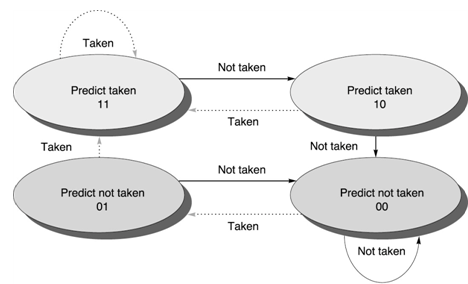
\includegraphics[width=1\textwidth]{figures/automato.png}
	\caption{Aut\^{o}mato finito descreve o comportamento do preditor de saltos \cite{493986}.}
	\label{fig:Fig_automato}
\end{figure}

\begin{figure}[ht]
	\centering
	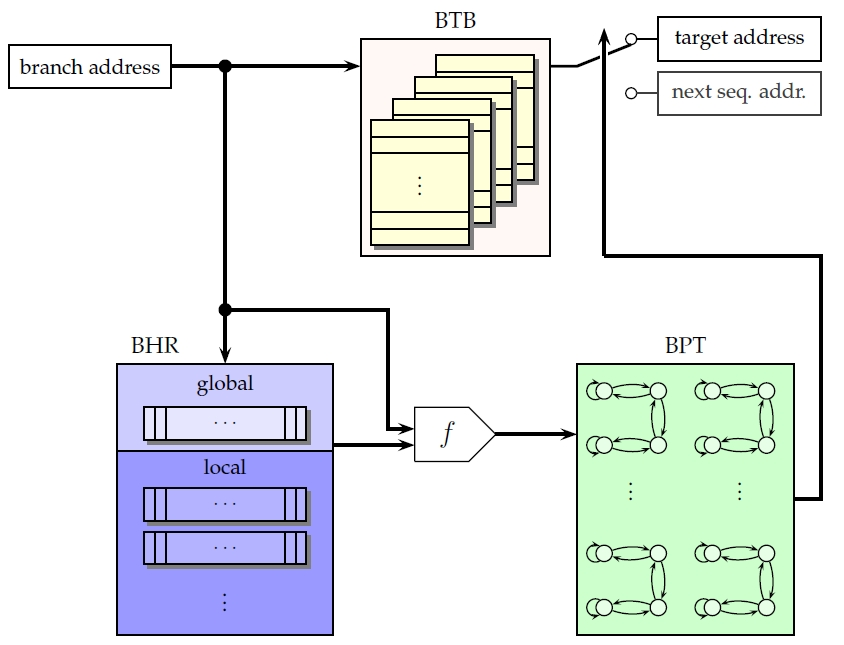
\includegraphics[width=.5\textwidth]{figures/btu.jpg}
	\caption{Unidade de predi\c{c}\~{a}o de saltos \cite{Jean-Pierre06predictingsecret}.}
	\label{fig:Fig_btu}
\end{figure}

\subsubsection*{Medi\c{c}\~{a}o direta de tempo}

A m\'{a}quina de estados que descreve as poss\'{i}veis decis\~{o}es da BTU possui um n\'{u}mero finito de estados; logo, o algoritmo que a descreve \'{e} determin\'{i}stico. O advers\'{a}rio pode assumir que a implementa\c{c}\~{a}o do RSA utilizou S\&M (\textit{Square-and-Multiply exponentiation algorithm}) e MM (\textit{Montgomery Multiplication algorithm} \cite{ECCBook_HankersonVanstone2004, 1197338}) e o BTU possui um aut\^{o}mato finito de apenas dois estados: salto tomado ou n\~{a}o tomado.

Seja $d$ a chave privada, vamos supor que o advers\'{a}rio conhece seus $i$ primeiros bits e est\'{a} tentando determinar $d_{i}$. Para qualquer mensagem $m$, o advers\'{a}rio pode simular as primeiras $i$ itera\c{c}\~{o}es e obter um resultado intermedi\'{a}rio que ser\'{a} a entrada da $(i+1)-$\textit{\'{e}sima} itera\c{c}\~{a}o. Ent\~{a}o ele gera quatro conjuntos distintos tais que:

\begin{align} \notag
	M_{1} = \left\lbrace m\ \vert\ d_{i} = 1 \rightarrow m\ causa\ missprediction\ durante\ MM\right\rbrace \\ \notag
	M_{2} = \left\lbrace m\ \vert\ d_{i} = 1 \rightarrow m\ causa\ hit\ durante\ MM\ \ \ \ \ \ \ \ \ \ \ \ \ \ \ \ \ \ \ \ \right\rbrace \\ \notag
	M_{3} = \left\lbrace m\ \vert\ d_{i} = 0 \rightarrow m\ causa\ missprediction\ durante\ MM\right\rbrace \\ \notag
	M_{4} = \left\lbrace m\ \vert\ d_{i} = 0 \rightarrow m\ causa\ hit\ durante\ MM\ \ \ \ \ \ \ \ \ \ \ \ \ \ \ \ \ \ \ \ \right\rbrace \\ \notag
\end{align}

O advers\'{a}rio calcula o tempo m\'{e}dio de execu\c{c}\~{a}o na multiplica\c{c}\~{a}o de Montgomery em cada conjunto $M_{i}$. Sendo $d_{i} = t, t \in \left\lbrace 0,1\right\rbrace $, a diferen\c{c}a dos tempos m\'{e}dios de execu\c{c}\~{a}o para o mesmo valor correto $t$ ser\~{a}o muito mais significativas do que a obtida dos outros dois conjuntos, pois, para o valor incorreto, os valores de tempo de cada multiplica\c{c}\~{a}o ter\~{a}o um caracter aleat\'{o}rio. Esse \'{e} o mesmo processo estat\'{i}stico da an\'{a}lise diferencial de pot\^{e}ncia. Portanto, se a diferen\c{c}a entre os tempos m\'{e}dios de $M_{1}$ e $M_{2}$ for muito mais significativa do que $M_{3}$ e $M_{4}$, ent\~{a}o o palpite correto \'{e} $d_{i} = 1$, e $d_{i} = 0$ caso contr\'{a}rio. 

Nesse ataque o advers\'{a}rio precisa saber de antem\~{a}o o estado do BPU antes do algoritmo de decripta\c{c}\~{a}o ser iniciado. Uma possibilidade de simples implementa\c{c}\~{a}o, por\'{e}m menos eficiente, seria realizar a an\'{a}lise supondo cada um dos quatro estados iniciais. A segunda abordagem consiste em for\c{c}ar o estado inicial do BPU de modo que nenhum endere\c{c}o de salto esteja no BTB. Essa abordagem ser\'{a} fundamentalmente a mesma utilizada em todos os ataques de predi\c{c}\~{a}o de salto listados a seguir.

\subsubsection*{For\c{c}ando BPU \`{a} mesma predi\c{c}\~{a}o assincronamente}

Unidades de processamento que permitem execu\c{c}\~{a}o concorrente de processos (SMT ou \textit{Simultaneous Multi-Threading} \cite{Silberschatz2004}) permitem que um advers\'{a}rio execute um processo espi\~{a}o simultaneamente ao programa de encripta\c{c}\~{a}o. Dessa forma, o advers\'{a}rio pode fazer com que o valor previsto dos saltos do encriptador nunca estejam no BTB; conseq\"{u}entemente, sempre ocorrer\'{a} um \textit{missprediction} quando o resultado correto, segundo a previs\~{a}o, seria que o salto fosse tomado. Comparado ao processo anterior, a an\'{a}lise diferencial seria similiar exceto pelo fato de que $d_{i} = 1$ em caso de \textit{hit} e $d_{i} = 0$ em caso de \textit{missprediction} durante o c\'{a}lculo de $m^{2} \bmod N$.

O processo espi\~{a}o remover do BTB o endere\c{c}o alvo de salto dos seguintes modos:
\begin{enumerate}
	\item (\textit{Total Eviction Method}: todas as entradas do BTB s\~{a}o expulsas.
	\item (\textit{Partial Eviction Method}): um conjunto de entradas do BTB \'{e} expulso.
	\item (\textit{Single Eviction Method}): apenas endere\c{c}o de interesse \'{e} expulso da tabela.
\end{enumerate}

Obviamente o primeiro m\'{e}todo \'{e} o de mais simples implementa\c{c}\~{a}o (assumindo que sejamos capazes de esvaziar todo o BTB entre duas itera\c{c}\~{o}es da exponencia\c{c}\~{a}o). O diferencial desse ataque \'{e} o advers\'{a}rio n\~{a}o ter que saber detalhes de implementa\c{c}\~{a}o da BPU para ser capaz de criar o processo espi\~{a}o e determinar quais s\~{a}o os bits da chave secreta.

\begin{figure}[ht]
	\centering
	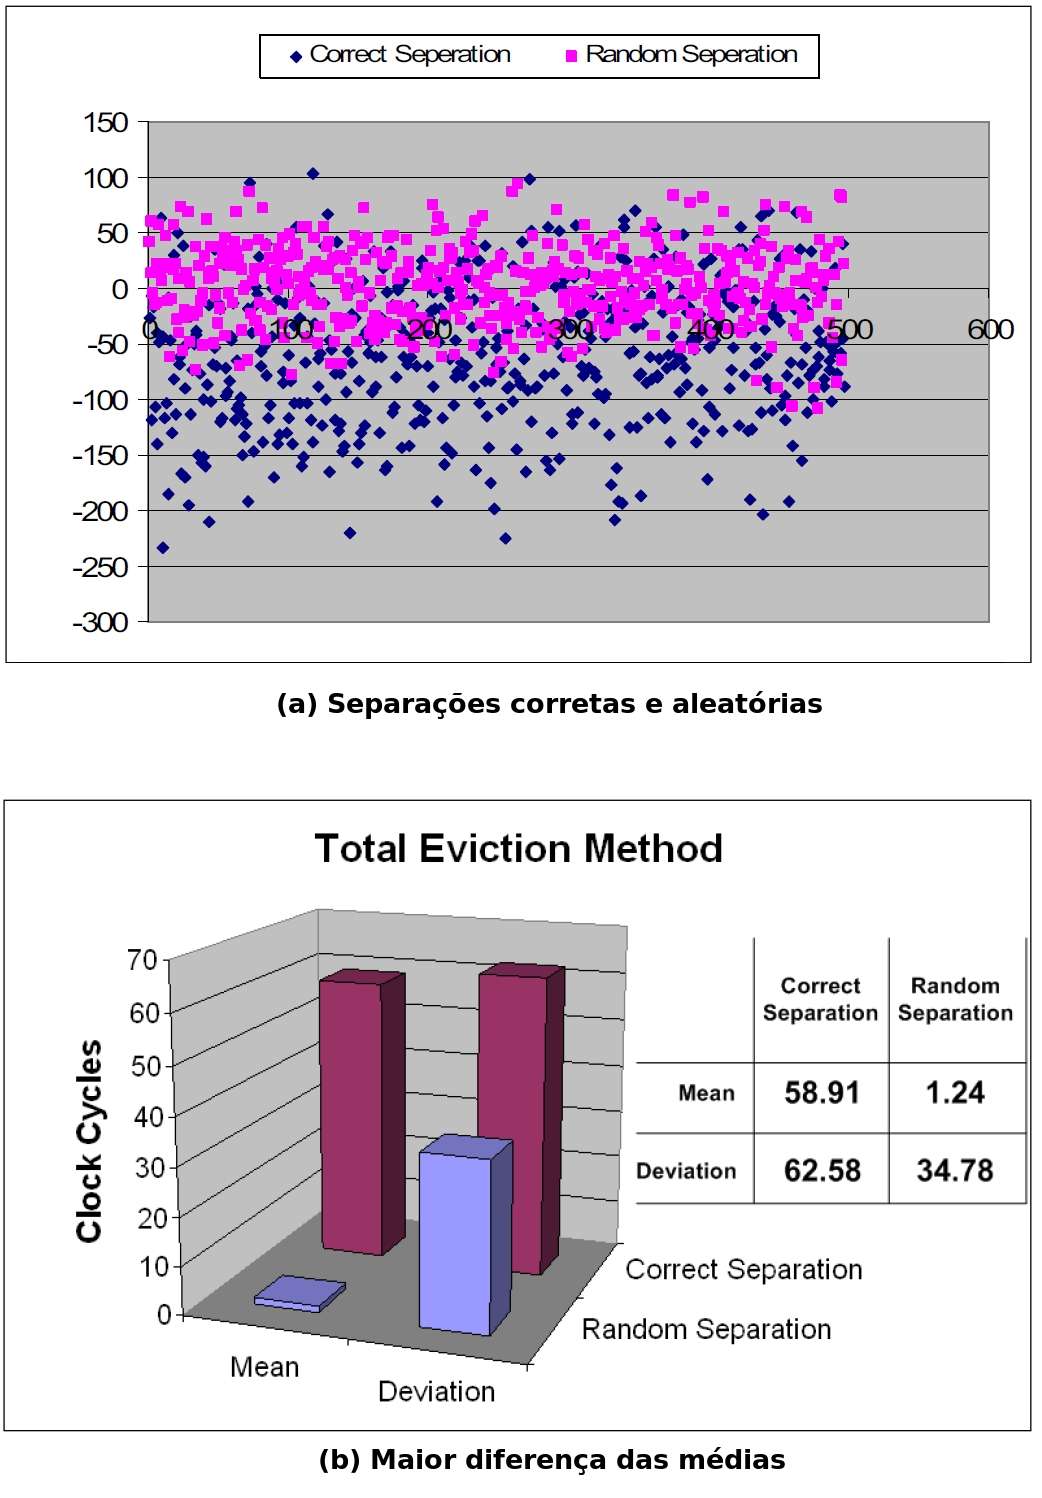
\includegraphics[width=.7\textwidth]{figures/totaleviction.jpg}
	\caption{Resultados pr\'{a}ticos do \textit{Total Eviction Method} \cite{Jean-Pierre06predictingsecret}.}
	\label{fig:Fig_totaleviction}
\end{figure}

Esse ataque foi aplicado sobre uma implementa\c{c}\~{a}o do RSA em OpenSSL vers\~{a}o 0.9.7, rodando sob uma workstation RedHat 3. Foram gerados 10 milh\~{o}es de blocos de mensagens aleat\'{o}rias e chaves aleat\'{o}rias de $512$ bits. As mensagens foram encriptadas e separadas segundo os crit\'{e}rios acima, sendo assumido como tomado o salto do pr\'{o}ximo bit desconhecido.
       
Na Figura ~\ref{fig:Fig_totaleviction} (a), o eixo $x$ corresponde aos bits do expoente de 2 at\'{e} 511, sendo que cada coordenada $x_{i}$ apresenta os valores das m\'{e}dias das separa\c{c}\~{o}es correta e a m\'{e}dia das separa\c{c}\~{o}es aleat\'{o}rias, denotadas respectivamente por $\mu_{Y_{i}}$ e $\mu_{X_{i}}$. Analizando todos os pares $(\mu_{Y_{i}}, \mu_{X_{i}})$, o advers\'{a}rio verifica  qual deles teve a diferen\c{c}a mais significativa (Figura ~\ref{fig:Fig_totaleviction} (b)) e utiliza seus respectivos desvios padr\~{o}es para determinar o desvio da diferen\c{c}a das m\'{e}dias

\begin{align}\notag
    \mu_{Z} &= \mu_{Y} - \mu_{X} = 58.91 - 1.24 = 57.67\\\notag
    \sigma_{Z} &= \sqrt{ \sigma_{Y}^{2} + \sigma_{X}^{2}} = \sqrt{ 62.58^{2} - (34.78)^{2}} = 71.60\\ \notag
\end{align}

Sempre que o advers'{a}rio encontrar $Z > 0$, ele ir\'{a} supor que seu palpite do valor do \textit{bit} foi correta. O grau de certeza que o advers\'{a}rio pode ter nessas decis\~{o}es pode ser medido atrav\'{e}s da probabilidade:

\begin{align}
    Pr[Z > 0] = \phi(\dfrac{0 - \mu_{Z}}{\sigma_{Z}}) = \phi(-0.805) = 0.79\notag
\end{align}

Portanto, a probabilidade de suas decis\~{o}es estarem corretas para essas medidas \'{e} de quase 80\%, viabilizando o advser\'{a}rio obter o restante da chave por for\c{c}a bruta.

\subsubsection{Limitações}

\subsubsection{Impacto em IoT}

\subsection{Canal lateral de potência}

\subsubsection{Características gerais}
Em um ataque sobre o canal lateral de pot\^{e}ncia, o advers\'{a}rio analisa sutis varia\c{c}\~{o}es no consumo de energia el\'{e}trica de um dispositivo cujo \textit{hardware} implementa um algoritmo criptogr\'{a}fico (sensores RFID, \textit{smartcards}, \textit{SIM cards}, etc).

Opera\c{c}\~{o}es com dados sens\'{i}veis geram alter\c{c}\~{o}es na corrente ou tens\~{a}o da alimenta\c{c}\~{a}o do dispositivo, permitindo extrair parcialmente (ou mesmo integralmente) a chave criptogr\'{a}fica e outras informa\c{c}\~{o}es  sens\'{i}veis. O primeiro ataque dessa natureza foi apresentado por \cite{Kocher:1999:DPA:646764.703989}, tamb\'{e}m autor da c\'{e}lebre pesquisa precursora sobre \textit{time attacks} \cite{Kocher96}. 

\paragraph{Comparação entre canais laterais de potência e de tempo}

\subsubsection{Ataque de potência simples (SPA)}
A tecnologia de semicondutores dominante em microprocessadores, mem\'{o}rias e dispositivos embarcados \'{e} a CMOS   \cite{sedra:1997}, sendo inversores l\'{o}gicos sua unidade b\'{a}sica de constru\c{c}\~{a}o. Como dispositivos utilizam fontes constantes de tens\~{a}o, a pot\^{e}ncia consumida varia de acordo com o fluxo de sinais nos componentes, e esses de acordo com as opera\c{c}\~{o}es realizadas. Se esse consumo de pot\^{e}ncia for monitorado com aux\'{i}lio de um oscilosc\'{o}pio poderemos estabelecer um rastro de consumo de pot\^{e}ncia (\textit{power trace}) a cada ciclo do dispositivo.

\subsubsection{An\'{a}lise simples de pot\^{e}ncia sobre ECDSA}
Uma das rotinas mais executadas em dispositivos que utilizam ECC s\~{a}o os algoritmos de assinatura digital de curvas el\'{i}pticas (\textit{ECDSA} ou \textit{Elliptic Curve Digital Signature Algorithm}), tendo como opera\c{c}\~{a}o central a multiplica\c{c}\~{a}o de um ponto por um escalar (Algoritmo 9).

\floatname{algorithm}{Algoritmo}
\begin{algorithm}[H]
\caption{Binary NAF method for scalar multiplication}
\begin{algorithmic}
    \REQUIRE $P \in E(\mathbb{F}_p), k \in \mathbb{N}$
    \ENSURE $Q = kP \in E(\mathbb{F}_p)$
    \STATE $(k_{l-1}, k_{l-2}, ..., k_{1}, k_{0}) \leftarrow NAF(k)$
    \STATE $Q \leftarrow \infty$
    \FOR {$j \leftarrow l - 2$ \TO $0$}
        \STATE $Q \leftarrow 2Q$
        \IF {$k_{i} = 1$}
            \STATE $Q \leftarrow Q + P$
        \ENDIF
        \IF {$k_{i} = -1$}
            \STATE $Q \leftarrow Q - P$
        \ENDIF
    \ENDFOR
    \RETURN $Q$
    \end{algorithmic}
\end{algorithm}

\begin{figure}[ht]
	\centering
	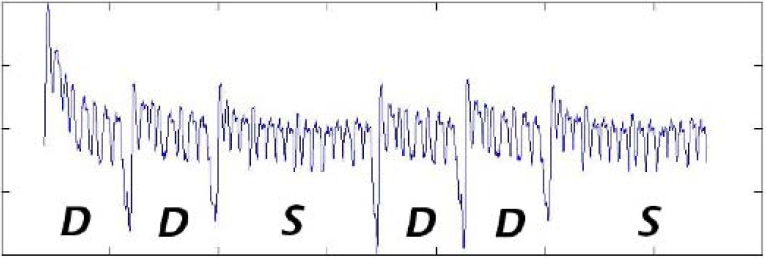
\includegraphics[width=.8\textwidth]{figures/spa1.jpg}
	\caption{Consumo de pot\^{e}ncia durante c\'{a}lculo de $kP$ \cite{ECCBook_HankersonVanstone2004}.}
	\label{fig:Fig5}
\end{figure}

O que torna a forma n\~{a}o adjacente de $k$ mais interessante do que sua representa\c{c}\~{a}o bin\'{a}ria \'{e} o fato da $NAF(k)$ possuir apenas $1/3$ de d\'{i}gitos n\~{a}o nulos. Conseq\"{u}entemente uma quantidade muito menor de adi\c{c}\~{o}es (linhas $04$ e $05$ do Algoritmo 8) s\~{a}o efetuadas.

Entretanto um advers\'{a}rio que soubesse que o dispositivo implementa um algoritmo \textit{ECDSA} poderia monitorar o consumo de pot\^{e}ncia do dispositivo utilizando um oscilosc\'{o}pio, obtendo o gr\'{a}fico mostrado na Figura~\ref{fig:Fig5}. No Algoritmo 9, vemos que adi\c{c}\~{o}es s\~{a}o realizadas apenas quando $k_{i} \neq 0$; logo, uma maior quantidade de pot\^{e}ncia \'{e} despendida para d\'{i}gitos n\~{a}o nulos. Portanto os intervalos curtos denominados $D$ correspondem a itera\c{c}\~{o}es em que $k_{i} = 0$, enquanto intervalos longos denominados $S$ correspondem a itera\c{c}\~{o}es em que $k_{i} \neq 0$. Essa informa\c{c}\~{a}o torna vi\'{a}vel descobrir a chave atrav\'{e}s de ataques por for\c{c}a bruta, pois apenas $1/3$ dos d\'{i}gitos s\~{a}o n\~{a}o nulos.

A solu\c{c}\~{a}o mais simples contra SPA consiste em inserir opera\c{c}\~{o}es redundantes no algoritmo de multiplica\c{c}\~{a}o (Algoritmo 10), de modo que a seq\"{u}\^{e}ncia de opera\c{c}\~{o}es elementares envolvidas sejam realizadas em igual propor\c{c}\~{a}o. Comparando o novo \textit{power trace} obtido (Figura~\ref{fig:Fig7}) n\~{a}o \'{e} poss\'{i}vel diferenciar adi\c{c}\~{o}es de multiplica\c{c}\~{o}es.

\floatname{algorithm}{Algoritmo}
\begin{algorithm}[H]
\caption{Binary NAF method for scalar multiplication resistant to SPA}
\begin{algorithmic}
    \REQUIRE $P \in E(\mathbb{F}_p), k \in \mathbb{N}$
    \ENSURE $Q = kP \in E(\mathbb{F}_p)$
    \STATE $(k_{l-1}, k_{l-2}, ..., k_{1}, k_{0}) \leftarrow NAF(k)$
    \STATE $Q \leftarrow \infty$\\
    \FOR {$i = l-1$ \TO $0$}
        \STATE $Q_{0} = 2Q_{0}$
        \STATE $Q_{1} = Q_{0} + P$
        \STATE $Q_{0} = Q_{k_{i}}$
    \ENDFOR
    \RETURN $Q$
    \end{algorithmic}
\end{algorithm}

\begin{figure}[ht]
	\centering
	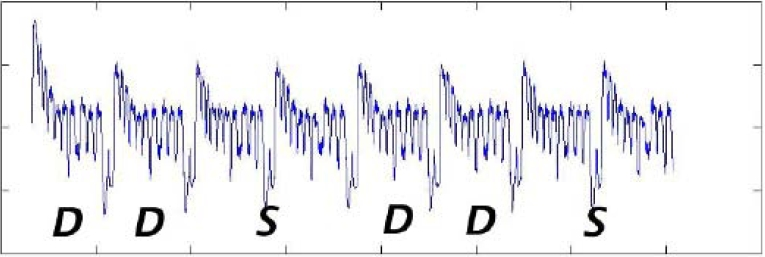
\includegraphics[width=.8\textwidth]{figures/spa2.jpg}
	\caption{Consumo de pot\^{e}ncia durante c\'{a}lculo de $kP$ \cite{ECCBook_HankersonVanstone2004}.}
	\label{fig:Fig7}
\end{figure}

\subsubsection{Ataque de potência diferencial (DPA)}
Quando a varia\c{c}\~{a}o do consumo de pot\^{e}ncia n\~{a}o \'{e} sens\'{i}vel o suficiente em rela\c{c}\~{a}o as opera\c{c}\~{o}es executadas por um dispositivo, o advers\'{a}rio pode monitorar como o consumo varia em rela\c{c}\~{a}o ao valor de uma determinada vari\'{a}vel. Nesse ataque, primeiramente detectamos uma vari\'{a}vel $V$, influenciada, durante um processo de decripta\c{c}\~{a}o ou assinatura digital, por um texto $m$ e uma por\c{c}\~{a}o desconhecida  da chave privada. A partir disso, definimos a fun\c{c}\~{a}o de sele\c{c}\~{a}o $V = f(k',m)$.

O advers\'{a}rio ent\~{a}o coleta milhares de \textit{power traces}, determinando indutivamente todos os bits que comp\~{o}em a chave privada atrav\'{e}s do c\'{a}lculo da derivada dessa fun\c{c}\~{a}o. Para cada bit $k'_{i}$ corretamente previsto obtemos uma derivada n\~{a}o nula para os valores de $k'$ e $m$, caso contr\'{a}rio a derivada \'{e} nula. O processo \'{e} repetido at\'{e} que cada $k'_{i}$ seja determinando \cite{ECCBook_HankersonVanstone2004}. Esse modelo de ataque \'{e} conhecido como An\'{a}lise Diferencial de Pot\^{e}ncia (DPA ou \textit{Differential Power Analysis}).


\subsection{An\'{a}lise diferencial de pot\^{e}ncia sobre ECDSA}
Ainda que o Algoritmo 10 tenha sido adotado, podemos aplicar um DPA sobre o processo de ECDSA. 

Determinada uma vari\'{a}vel $V$ cujo valor influencie o consumo de pot\^{e}ncia e uma fun\c{c}\~{a}o de sele\c{c}\~{a}o $f$ tal que $V = f(k', m)$ o advers\'{a}rio coleta milhares de \textit{power traces}, estima o tamanho que a por\c{c}\~{a}o $k'$ ocupa na chave privada e separa os dados coletados em dois grupos de acordo com o valor previsto de $V$.

No algoritmo de multiplica\'{c}\~{a}o de pontos da curva el\'{i}ptica (Algoritmo 1.6), suponha que Eve colete \textit{power traces} durante os c\'{a}lculos $kP_{1} , kP_{2} , ..., kP_{r}$ . Como $P_{1} , P_{2} , ..., P_{r}$ s\~{a}o p\'{u}blicos, ele precisa determinar apenas $k$.

\begin{center}
    \begin{tabular}{|c|c|c|c|c|}
	    \hline
		    \   & $Q_{0}$  & $Q_{0}$ & $k_{t-1}$ & $Q_{0} \leftarrow Q_{k_{t-1}}$\\
	    \hline
	        $1$ & $\infty$ &     $P$ &       $1$ & $P$\\
	    \hline
		    $2$ & ... & ... & ... & ...\\
	    \hline
		    $3$ & ... & ... & ...& ... \\
	    \hline
		    ... & ... & ... & ...& ... \\
	    \hline
    \end{tabular}

    Tabela 1.2. $k = (1, k_{t-2}, k_{t-3}, ..., k_{1}, k_{0})$.
\end{center}

Dado $Q_{0} = \infty$, o passo 2.1 \'{e} trivial e pode ser disting\"{u}ir da de uma opera\c{c}\~{a}o n\~{a}o trivial
atrav\'{e}s do power trace, logo o advers\'{a}rio pode facilmente identificar o bit mais a esquerda cujo valor e 1. Tomando $k_{t-1}= 1$, na segunda itera\c{c}\~{a}o do algoritmo temos que $Q_{0} = 2P$ (se $k_{t-2} = 0$) ou $Q_{0} = 3P$ (se $k_{t-2} = 1$).

\begin{center}
    \begin{tabular}{|c|c|c|c|c|}
	    \hline
		    \   & $Q_{0}$  & $Q_{0}$ & $k_{t-1}$ & $Q_{0} \leftarrow Q_{k_{t-1}}$\\
	    \hline
	        $1$ & $\infty$ &     $P$ &       $1$ & $P$\\
	    \hline
		    $2$ & $2P$ & $4P$ & $\color{blue}{?}$ & $\color{blue}{?}$ \\
	    \hline
		    $3$ & ... & ... & ...& ... \\
	    \hline
		    ... & ... & ... & ...& ... \\
	    \hline
    \end{tabular}

    Tabela 1.3. $k = (1, k_{t-2}, k_{t-3}, ..., k_{1}, k_{0})$.
\end{center}

Conseq\"{u}entemente, na terceira itera\c{c}\~{a}o, o valor $4P$ ser computado apenas se $k_{t-2} = 0$. Definindo $k' = k_{t-2}$ e $m = P_{i}$ ($i$-\'{e}simo bit do ponto $4P = (4P_{1} , 4P_{2} , ..., 4P_{i} , ..., 4P_{r} , )$), a fun\c{c}\~{a}o seletora calcula o valor do bit $4P_{i}$.

\begin{center}
    \begin{tabular}{|c|c|c|c|c|}
	    \hline
		    \   & $Q_{0}$  & $Q_{0}$ & $k_{t-1}$ & $Q_{0} \leftarrow Q_{k_{t-1}}$\\
	    \hline
	        $1$ & $\infty$ &     $P$ &       $1$ & $P$\\
	    \hline
		    $2$ & $2P$ & $4P$ & $\color{red}{0}$ & $2P$ \\
	    \hline
		    $3$ & $\color{red}{4P}$ & $6P$ & ...& ... \\
	    \hline
		    ... & ... & ... & ...& ... \\
	    \hline
    \end{tabular}

    Tabela 1.4. $k = (1, \color{red}{0}$$,\ $$k_{t-3}, ..., k_{1}, k_{0})$.
\end{center}

Se o gr\'{a}fico do consumo de pot\^{e}ncia da fun\c{c}\~{a}o apresentar picos, ent\~{a}o $k_{t-2} = 0$, caso contr\'{a}rio $k_{t-2} = 1$.
Esse processo \'{e} repetido at\'{e} todos os bits de $k$ serem determinados \cite{ECCBook_HankersonVanstone2004}.

Se a curva el\'{i}ptica for gerada sobre um $\mathbb{F}_{p}$ de caracter\'{i}stica superior a 3, podemos usar um sistema misto de representa\c{c}\~{a}o de coordenadas no qual $P$ seja representado em um sistema de coordenadas afins, enquanto $Q_{0}$ e $Q_{1}$ s\~{a}o representados em coordenadas jacobianas \cite{ECCBook_HankersonVanstone2004}.

Se $P = (x,y)$ no sistema afim, ap\'{o}s a primeira atribui\c{c}\~{a}o $Q_{1} \leftarrow P$ ter\'{i}amos $ Q_{1} = (x : y : 1)$. Ent\~{a}o, $Q_{1}$ seria aleatorizado com $(\lambda^{2}x, \lambda^{3}y, \lambda)$ e o algoritmo procederia como o usual. Desse modo o advers\'{a}rio estaria impedido de realizar predi\c{c}\~{o}es baseadas no valor de um bit espec\'{i}fico $4P_{i}$ em sistemas de coordenadas jacobianas aleatorizadas.

\subsubsection{High-order DPA}
Uma variação do ataque de potência diferencial é o \textit{high-order} DPA (HODPA), esse ataque é baseado em um conjunto de propriedades estatísticas do sinal de potência. Para obter uma melhor taxa de acerto dos \textit{bits} da chave é necessário uma quantidade maior de amostras. Além disso, existe uma complexidade maior durante a implementação desse ataque \cite{benedikt:2009:228}.

Um ponto importante a ser observado é que esse ataque possui a capacidade de sobrepor a resistência de uma contramedida de \textit{masking} e obter os \textit{bits} da chave. Isso é possível pela análise tanto do valor mascarado como da própria máscara criando uma relação entre ambos. Um problema encontrado na utilização desse ataque é a identificação de em qual tempo é necessário obter o sinal referente ao valor mascarado ou a máscara.

\subsubsection{Template attacks}
O ataque que será apresentado, \textit{Template Attack} (TA), utiliza amostras de potência elétrica para executar uma análise na tentativa de obter os \textit{bits} da chave privada. O mesmo é considerado o mais poderoso dentre os ataques de potência diferencial. Existe uma divisão em duas fases do ataque sendo: a fase de construção e a fase de correlação. A primeira gera um \textit{template} de um padrão obtido no dispositivo alvo. Na segunda é analisada a correlação entre o \textit{template} gerado e as amostras obtidas durante a execução do dispositivo \cite{ozgen:2016}. Esse ataque pode ser combinado com algoritmos de classificação para diferenciar valores da chave e o restante como é proposto no trabalho de \cite{ozgen:2016}. Uma outra opção é a utilização de algoritmos de reconhecimento de padrões com aprendizado de máquina.
